% vim:syntax=tex

In this section we describe the design of a case study in which we
explore the relationship between ownership and linguistic topics in source code.
We describe the case study using the Goal-Question-Metric approach~\cite{Basili-etal:94}.
%The data for the case study is available in this paper's online
%appendix\footnote{\url{http://software.eng.ua.edu/data/ownership-topics}}.

\subsection{Definition and Context}

Our \textit{goal} is to explore the relationship between changeset topics and snapshot topics.
The \textit{quality focus} of the study is on informing development decisions and policy changes
that could lead to software with fewer defects.
The \textit{perspective} of the study is of a researcher, developer, or project manager who wishes
to gain understanding of the concepts or features implemented in the source code.
The \textit{context} of the study spans the version histories of four open source systems.

Toward achievement of our goal, we pose the following research questions:
\begin{description}[font=\itshape\mdseries,leftmargin=10mm,style=sameline]
    \item[RQ1] Do changeset- and snapshot-based corpora express the same terms?
    \item[RQ2] Are topic models trained on changesets more distinct than topic models trained on a snapshot?
\end{description}
Basically, we want to know whether topic modeling changesets is as good as, or better than, topic modeling a snapshot.

In the remainder of this section we introduce the subjects of our study,
describe the setting of our study, and report our data collection and analysis procedures.

%%%%%%%%%%%%%%%%%%%%%%%%%%%%%%%%%%%%%%%%%%%%%%%%%%%%%%%%%%%%%%%%%%%%%%%%

\subsection{Subject software systems}

The four subjects of our study ---
Apache \ant\footnote{\url{http://ant.apache.org/}},
\aspectj\footnote{\url{http://eclipse.org/aspectj/}},
\jodatime\footnote{\url{http://www.joda.org/joda-time/}},
and \postgres\footnote{\url{http://www.postgresql.org/}}
--- vary in language, size and application domain.
\ant\ is a library and command-line tool for managing builds,
\aspectj\ is an aspect-oriented programming extension for the Java language,
\jodatime\ is a library for replacing the Java standard library \texttt{date} and \texttt{time} classes,
and \postgres\ is an object-relational database management system.
Each system is stored in a Git repository, and the developers of each system use descriptive commit messages.
Further, the developers store bug reports in an issue tracker.
All systems are written in Java with the exception of \postgres,
which is written in C. Table~\ref{tab:systems} outlines the releases for
each system studied.

%%%%%%%%%%%%%%%%%%%%%%%%%%%%%%%%%%%%%%%%%%%%%%%%%%%%%%%%%%%%%%%%%%%%%%%%

\subsection{Setting}

\begin{figure*}[!th]
    \centering
    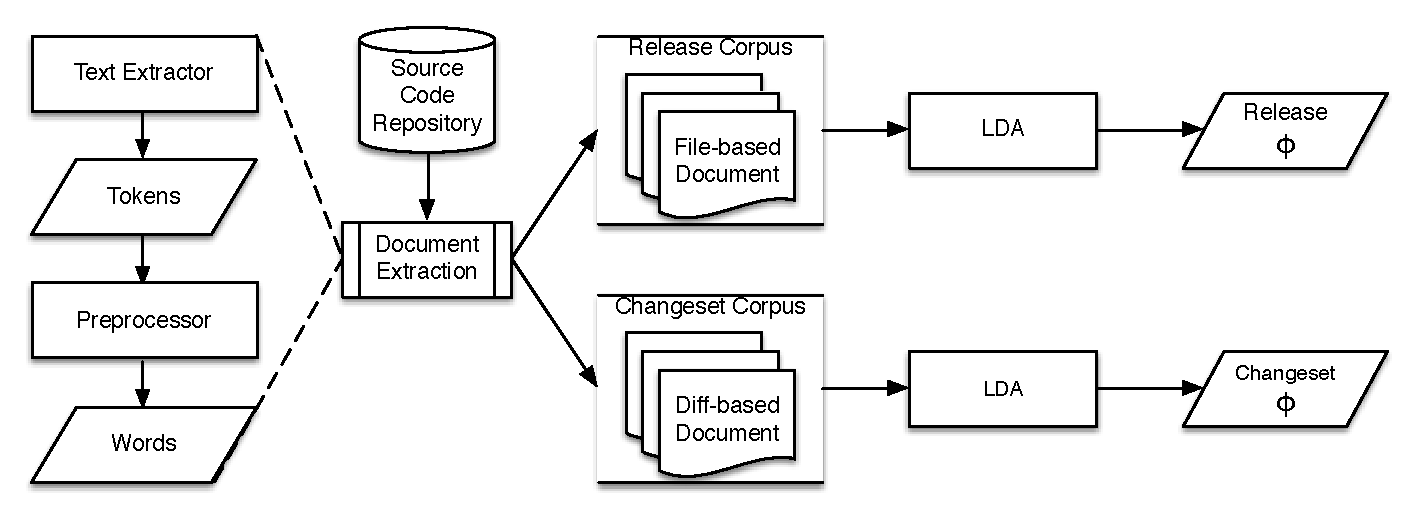
\includegraphics[width=.75\textwidth]{changeset}
    \caption{Extraction and Modeling Process}
    \label{fig:process}
\end{figure*}

Our document extraction process is shown on the left side of Figure~\ref{fig:process}.
We implemented our document extractor in Python v2.7
using the Dulwich library\footnote{\url{http://www.samba.org/~jelmer/dulwich/}} %\footnote{\url{https://pypi.python.org/pypi/dulwich}}
We extract documents from both a snapshot of the repository at a tagged
release and each commit reachable from that tag's commit.
The same preprocessing steps are employed on all documents extracted.

For our document extraction from a release,
we simply use the entire contents of the document.
Unlike previous methods, %\needcite,
we do not parse the source code documents for classes, methods, and so on.
%We do this because so-and-so-I-forget\needcite,
%but also it leaves our technique language-independent.
We do this to leave our technique language-independent,
and to also allow for a fair comparison between the two approaches.
Special characters such as braces and semicolons will be removed during
preprocessing.

To extract text from the changesets, we look at the output of viewing
the \texttt{git diff} between two commits.
Figure~\ref{fig:diff} shows an example of what a changeset might look
like in Git.
In our changeset text extractor, we only extract text from removed or added lines.
Context and metadata lines are ignored.
%Figure~\ref{fig:diffdocument} shows what words would be extracted to make up the document without preprocessing
%from the change shown in Figure~\ref{fig:diff}.
Note that we do not consider what type of document the text originates from,
only that it is text changed by the commit.

%Our document preprocessor implements the transformations described in Section~\ref{sec:preprocessing}.
%We filter \texttt{java.lang} class names before splitting tokens.
After extracting tokens, we split them based on camel case, underscores, and non-letters.
We normalize to lower case before filtering English stop words~\cite{StopWords}, Java keywords, and words shorter than three characters long.
We do not stem.


For our model generation, we use the open source Python library Gensim~\cite{Gensim}.
Gensim's LDA implementation is based on the Online LDA by Hoffman et al.~\cite{Hoffman-etal:2010}
and uses variational inference instead of a Collapsed Gibbs Sampler.
Unlike Gibbs sampling, in order to ensure that the model converges for each document,
we allow LDA to see each document $10$ times by setting Gensim's initialization parameter \texttt{passes} to this value.
We set the following LDA parameters for all four systems:
$100$ topics ($K$),
a symmetric $\alpha=0.01$,
$\beta$ is left as a default value of $1/K$ (also $0.01$).


\begin{figure}[ht]
\centering
\footnotesize
\begin{lstlisting}[language=diff, basicstyle=\ttfamily]
diff --git a/lao b/tzu
index 635ef2c..5af88a8 100644
--- a/lao
+++ b/tzu
@@ -1,7 +1,6 @@
-The Way that can be told of is not the eternal Way;
-The name that can be named is not the eternal name.
 The Nameless is the origin of Heaven and Earth;
-The Named is the mother of all things.
+The named is the mother of all things.
+
 Therefore let there always be non-being,
   so we may see their subtlety,
 And let there always be being,
@@ -9,3 +8,6 @@ And let there always be being,
 The two are the same,
 But after they are produced,
   they have different names.
+They both may be called deep and profound.
+Deeper and more profound,
+The door of all subtleties!
\end{lstlisting}
\caption{Example of a \texttt{git diff}. Black or blue lines denote metadata about the change, red lines (beginning with a single \texttt{-}) denote line removals, and green lines (beginning with a single \texttt{+}) denote line additions.}
\label{fig:diff}
\end{figure}

\begin{comment}
\begin{figure}[ht]
\em
\footnotesize
The Way that can be told of is not the eternal Way;
The name that can be named is not the eternal name.
The Named is the mother of all things.
The named is the mother of all things.
They both may be called deep and profound.
Deeper and more profound,
The door of all subtleties!
\caption{An example extracted changeset document before preprocessing}
\label{fig:diffdocument}
\end{figure}
\end{comment}

%%%%%%%%%%%%%%%%%%%%%%%%%%%%%%%%%%%%%%%%%%%%%%%%%%%%%%%%%%%%%%%%%%%%%%%%

\subsection{Data Collection and Analysis}

We create two corpora for each of our four subject systems.
We then used LDA to model the documents into topics.

To answer RQ1, we investigate the term frequency in each corpus.
We create two distributions from all unique terms from both corpora.
That is, each vector is of the same length and contain zero values for terms not in its respective corpus.
We measure the similarity of the two word-vectors using cosine distance.

To answer RQ2, we follow Thomas et al.~\cite{Thomas-etal:2011} 
and use topic distinctness to evaluate our topic models.
Distinct topics are topics with dissimilar word probabilities to all other topics in the model.
Using this metric will also allow a comparison to the results of Thomas et al.~\cite{Thomas-etal:2011}. 
Topic distinctness has also been shown to be an effective measure for qualitative
comparison of topic models in context of visualization~\cite{Wei-etal:2010, Chuang-etal:2012}.
Although Chang et al.~\cite{Chang-etal:2009} conclude that evaluating topic models
should depend on real-world tasks over metrics,
we argue that the positive results from using topic distinctness for visualization
techniques qualifies the metric for this exploratory study.

\begin{comment}
``Traditional metrics are, indeed, negatively correlated with the
measures of topic quality developed in this paper.  Our measures enable
new forms of model selection and suggest that practitioners developing
topic models should thus focus on evaluations that depend on real-world
task performance rather than optimizing likelihood-based measures.''~\cite{Chang-etal:2009}
\end{comment}


Thomas et al.\ define topic distinctness (TD) of a topic $z_i$ as the mean
Kullback-Leibler (KL) divergence between the vectors $z_i$ and $z_j$, $\forall j \neq i$:
\begin{equation}
TD(\phi_{z_i}) =
\frac{1}{K - 1}
\sum_{j=1,j \neq i}^{K}
KL(\phi_{z_i}, \phi_{z_j})
\label{eq:topicdistinctness}
\end{equation}

We score the overall topic distinctness of a model $\phi$ as the mean of
its topic distinctness scores, $\forall z \in \phi$.

\begin{comment}
\begin{equation}
TD(\phi) =
\frac{1}{K - 1}
\sum_{i=1}^{K}
TD(\phi_{z_i})
\label{eq:overalltopicdistinctness}
\end{equation}
\end{comment}


%%%%%%%%%%%%%%%%%%%%%%%%%%%%%%%%%%%%%%%%%%%%%%%%%%%%%%%%%%%%%%%%%%%%%%%%

\subsection{Results}

\begin{table*}[ht]
\renewcommand{\arraystretch}{1.3}
\footnotesize
\centering
\caption{Subject systems version and corpora description}
\begin{tabular}{lll rr rr rr}
    \toprule
            & Release & Commit & Release No.  & Changeset No. & Release No.    & Changeset No.  & Release No.    & Changeset No.\\
     System    & Version & SHA  & Documents   & Documents    & Unique Terms  & Unique Terms  & Total Terms   & Total Terms \\
    \midrule
    \ant        & 1.9.4   & 1c927b15 & 2208      & 12996     & 17986         & 74681         & 1066446       & 11801353 \\
    \aspectj    & 1.8.0   & 5a5bef1e & 10130     & 7650      & 22855         & 25071         & 4825289       & 10583008 \\
    \jodatime   & 2.3     & b0fcbb95 & 402       & 1750      & 9298          & 11385         & 493131        & 5541330 \\
    \postgres  & 9.3.4   & d4f8dde3 & 4080      & 36870     & 84591         & 164703        & 6644409       & 59850328 \\
    \bottomrule
\end{tabular}
\label{tab:systems}
\end{table*}

RQ1 asks whether a corpus generated from changesets have similar terms
as a corpus generated from a release.
We expected to find that set of unique terms in the changeset corpus to be
a superset of the set of unique terms in the release corpus.
Interestingly, this holds true for \jodatime\ and \aspectj,
but not for \ant\ and \postgres.
Further inspection shows that 2 terms appear in the \ant\ release corpus that do not appear in the changeset corpus,
and 19 terms appear in \postgres's respective corpora.
However, these anomalies appear to have been file encoding errors that
had been introduced into the version history.
For example, one of the terms for \ant\ was \texttt{rapha}. This is due
to an encoding error in the \texttt{KEYS} files for a developer named
``Rapha\"{e}l Luta''.

To answer RQ1, we created two word distributions that represented the unique
terms from both corpora for each system.
Figure~\ref{fig:antdist1} shows the normalized distribution of the \ant\ release corpus.
Likewise, Figure~\ref{fig:antdist2} shows the distribution of the \ant\ changeset corpus.
We measure the differences between the two distributions using the simple
cosine distance. For \ant, we had the lowest cosine distance of $0.00396$.
\aspectj\ and \jodatime\ have similar distances to another of $0.06929$ and
$0.06540$. \postgres\ had the highest, at an astounding $0.33957$.

%
% At this point, I would love to do a stats test. But I am way too tired
% to figure that out because I am butts at stats
%

\begin{figure*}[ht]
\centering
\begin{subfigure}[b]{0.4\textwidth}
    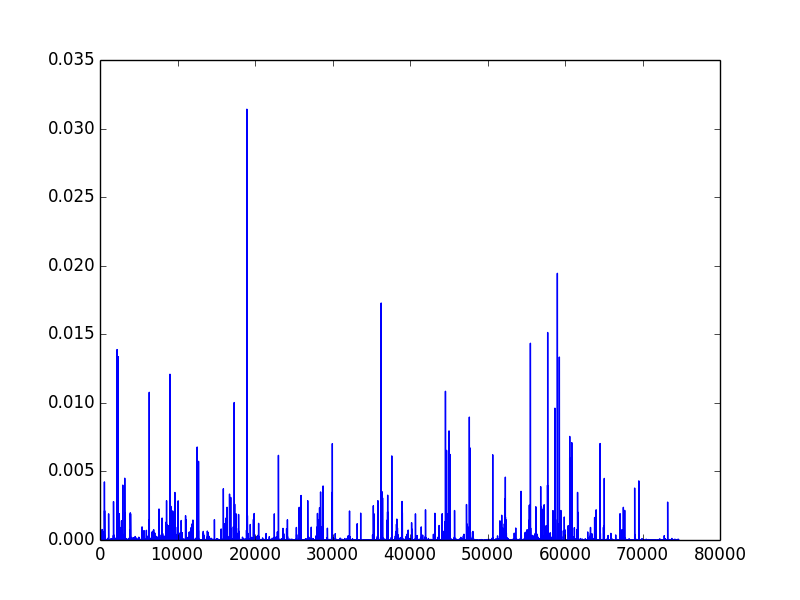
\includegraphics[width=\textwidth]{dist1}
    \caption{Normalized distribution of the release corpus}
    \label{fig:antdist1}
\end{subfigure}
\begin{subfigure}[b]{0.4\textwidth}
    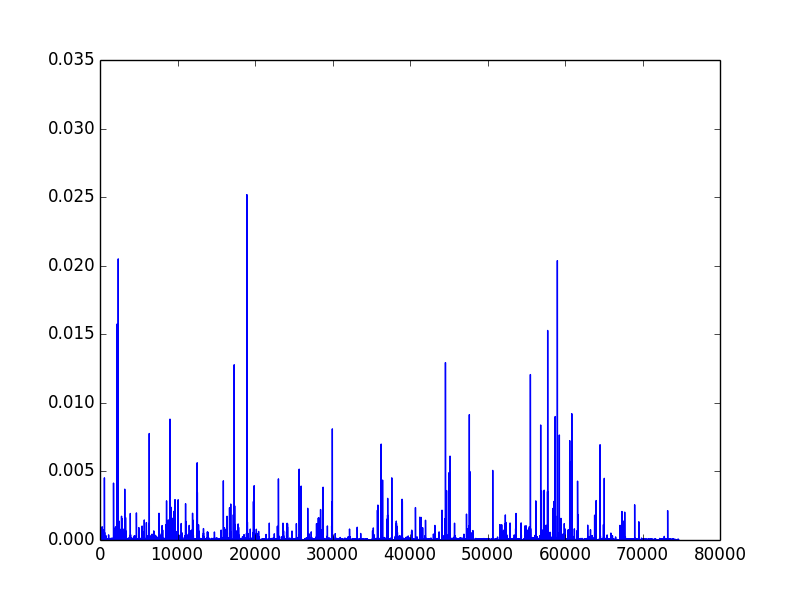
\includegraphics[width=\textwidth]{dist2}
    \caption{Normalized distribution of the changeset corpus}
    \label{fig:antdist2}
\end{subfigure}
\caption{Comparison of \ant\ word distributions}
\end{figure*}


RQ2 asks if topic models trained on changeset corpora produce more distinct
topics.
We expected to find that they would since ``popular'' words would become
more prevalent in the corpus from receiving several changes.
Table~\ref{tab:tdscores} shows our topic distinctness scores for each system.
Interestingly, this is true for \ant\ and \postgres,
but not for \jodatime\ and \aspectj.
We hypothesize this is because \ant\ and \postgres\ have a much richer history than \jodatime\ and \aspectj.
That is, \ant\ and \postgres\ have drastically more documents in their respective changeset corpora.
Table~\ref{tab:systems} shows the document count and term count for each system.


\begin{table}[h]
\renewcommand{\arraystretch}{1.3}
\footnotesize
\centering
\begin{tabular}{lrr}
    \toprule
    System      & Snapshot TD & Changeset TD \\
    \midrule
    \ant        & 2.31      & 3.17      \\
    \aspectj    & 3.75      & 2.78      \\
    \jodatime   & 1.34      & 1.03      \\
    \postgres   & 2.59      & 3.56      \\
    \bottomrule
\end{tabular}
\label{tab:tdscores}
\caption{Comparison of topic distinctness scores (RQ2)}
\end{table}
